\documentclass{beamer}
\usetheme{Madrid}
\usecolortheme{default}

% Packages
\usepackage{amsmath,amssymb}
\usepackage{graphicx}
\usepackage{siunitx}
\sisetup{per-mode=symbol}
\usepackage{gvv}
\usepackage{listings}
\usepackage{xcolor}

% Code style
\lstset{
  basicstyle=\ttfamily\scriptsize,
  breaklines=true,
  frame=single,
  numbers=left,
  numberstyle=\tiny,
  keywordstyle=\color{blue},
  commentstyle=\color{green!50!black},
  stringstyle=\color{red!60!black},
  showstringspaces=false
}

\title{Matrix 4.13.84}
\author{ai25btech11015 -- M Sai Rithik}
\date{}

\begin{document}
\maketitle

% Question
\begin{frame}
\frametitle{Question (4.13.84)}
Find the value of \(k\) such that the line
\[
\frac{x-4}{1}=\frac{y-2}{1}=\frac{z-k}{2}
\]
lies in the plane
\[
2x-4y+z=7.
\]
\end{frame}

% Parametric form
\begin{frame}
\frametitle{Parametric Form of Line}
The line can be written as
\[
\Vec{r}(t) = \myvec{x\\y\\z} = \Vec{p} + t\,\Vec{v},
\]
where
\[
\Vec{p} = \myvec{4\\2\\k}, \quad 
\Vec{v} = \myvec{1\\1\\2}.
\]

The plane can be written as
\[
\Vec{n}^T \Vec{r} = 7,
\quad \Vec{n} = \myvec{2\\-4\\1}.
\]
\end{frame}

% Conditions
\begin{frame}
\frametitle{Conditions for Line in Plane}
Substituting, we get
\[
\Vec{n}^T(\Vec{p} + t \Vec{v}) = 7,
\]
\[
\Vec{n}^T \Vec{p} + t\,\Vec{n}^T \Vec{v} = 7.
\]

For this to hold for all \(t\):
\begin{align}
\Vec{n}^T \Vec{v} &= 0, \\
\Vec{n}^T \Vec{p} &= 7.
\end{align}
\end{frame}

% Step 1 calculation
\begin{frame}
\frametitle{Step 1: Direction Condition}
\[
\Vec{n}^T \Vec{v}
= \begin{bmatrix}2 & -4 & 1\end{bmatrix}
\myvec{1\\1\\2}
= 2(1) + (-4)(1) + 1(2) = 0.
\]

Thus, the condition is satisfied automatically.
\end{frame}

% Step 2 calculation
\begin{frame}
\frametitle{Step 2: Point Condition}
\[
\Vec{n}^T \Vec{p}
= \begin{bmatrix}2 & -4 & 1\end{bmatrix}
\myvec{4\\2\\k}
= 8 - 8 + k = k.
\]

Equating,
\[
k = 7.
\]
\end{frame}

% Final Answer
\begin{frame}
\frametitle{Final Answer}
\[
\boxed{k = 7}
\]

\begin{figure}[h!]
    \centering
    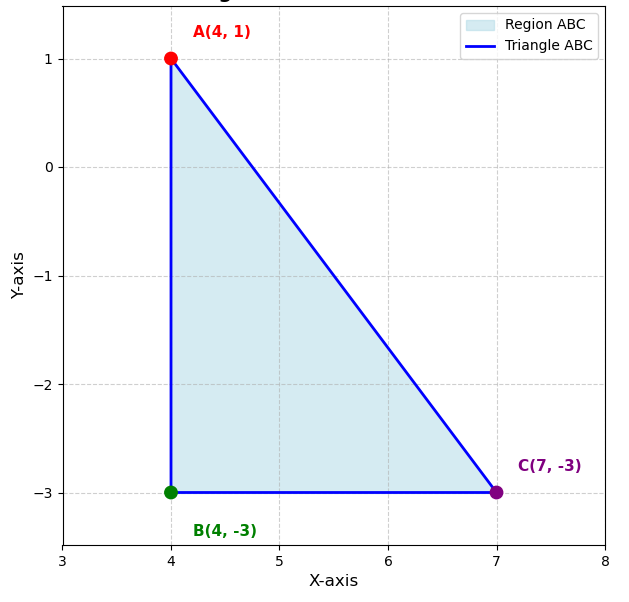
\includegraphics[width=0.65\linewidth]{figs/fig.png}
    \caption{Line lying in the plane}
\end{figure}
\end{frame}

\end{document}
